\documentclass[11pt,a4paper]{article}
\usepackage[margin=22mm]{geometry}
\usepackage{amsmath,amssymb,graphicx,booktabs,array,tabularx}
\usepackage[table]{xcolor}
\usepackage{caption,fancyhdr,hyperref}
\definecolor{navy}{HTML}{183153}
\definecolor{blue}{HTML}{2369A8}
\definecolor{pale}{HTML}{EEF4F9}
\definecolor{valid}{HTML}{D5E8F5}
\hypersetup{colorlinks=true,linkcolor=blue,urlcolor=blue,pdftitle={Homework 1: Risk Minimization and Model Selection}}
\graphicspath{{results/figures/}}
\setlength{\parindent}{0pt}
\setlength{\parskip}{6pt}
\renewcommand{\arraystretch}{1.25}
\captionsetup{font=small,labelfont=bf}
\pagestyle{fancy}
\fancyhf{}
\fancyhead[L]{\small\textcolor{navy}{PREDICTIVE LEARNING / HOMEWORK 1}}
\fancyfoot[L]{\small Risk minimization and model selection}
\fancyfoot[R]{\thepage}
\setlength{\headheight}{15pt}
\newcommand{\panel}[2]{\begin{minipage}[t]{0.49\linewidth}\centering\includegraphics[width=\linewidth]{#1}\par\small #2\end{minipage}}
\newcommand{\train}{\cellcolor{pale}T}
\newcommand{\val}{\cellcolor{valid}\textbf{V}}
\begin{document}
{\LARGE\bfseries\color{navy} Homework 1}\par
{\Large Risk Minimization and Model Selection}\par
\textcolor{blue}{Problems 2.7, 2.8, 2.11 and 2.12}

\section*{Overview}
This report studies two related questions: how to select model complexity from limited training data, and how to assess predictions on observations not used for fitting. Problems 2.7 and 2.8 use nearest-neighbor classification across election years. Problems 2.11 and 2.12 compare algebraic and cosine regression models using a complexity-adjusted criterion and five-fold validation.

\begin{center}\small
\begin{tabularx}{\linewidth}{l >{\raggedright\arraybackslash}X >{\raggedright\arraybackslash}X}
\toprule
Problem & Experimental design & Main result\\\midrule
2.7 & Train on 2004; test on 2000 & $k=7$; test accuracy $49.02\%$\\
2.8 & Train on 2000; test on 2004 & $k=7$; test accuracy $56.86\%$\\
2.11 & Select $m$ using Schwartz & Algebraic $m=1$; cosine $m=0$\\
2.12 & Five-fold evaluation & Mean MSE: cosine $0.20392$; algebraic $188.69045$\\
\bottomrule
\end{tabularx}\end{center}

\section*{Data and reproducibility}
The election files each contain 51 observations: the 50 states and Washington, D.C. Only obesity percentage is used as an input feature. The response is the supplied Democratic (D) or Republican (R) election label. Obesity itself is not the prediction target.

\begin{center}\begin{tabular}{lrrrr}
\toprule
Year & Observations & D & R & Mean obesity (\%)\\\midrule
2000 & 51 & 21 & 30 & 19.10\\
2004 & 51 & 19 & 32 & 22.39\\\bottomrule
\end{tabular}\end{center}

For regression, a new sample of ten observations is generated with NumPy's \texttt{default\_rng(42)}:
\begin{equation}
x_i\sim\mathcal U(0,1),\qquad
y_i=x_i^2+0.1x_i+\varepsilon_i,\qquad
\varepsilon_i\sim\mathcal N(0,0.5^2).
\end{equation}
Both regression families use this same sample. The true curve is shown only for interpretation; it is not used when fitting coefficients or selecting $m$.

\textbf{Implementation basis.} Results and figures correspond to the current HW1 implementation and saved tables. KNN uses Euclidean distance, uniform votes and \texttt{algorithm='brute'}. The separate exploratory \texttt{auto} run is not substituted into these results. Original row order and labels are preserved, including the supplied 2004 Hawaii label R. All election scores therefore evaluate the supplied labels.

\textbf{Source files.} Data: \texttt{data/}; algorithms: \texttt{src/}; numerical results: \texttt{results/tables/}; figures: \texttt{results/figures/}. The regression sample is newly generated and is not claimed to reproduce the textbook's exact observations.

\clearpage
\section*{Problems 2.7 and 2.8: KNN classification}
\subsection*{Method and selection rule}
For one-dimensional obesity inputs, the distance is $d(x,x_i)=|x-x_i|$. The $k$ nearest training observations vote uniformly for D or R. Every $k\in\{1,\ldots,50\}$ is assessed by leave-one-out cross-validation (LOOCV) within the training year:
\begin{equation}
\widehat R_{\mathrm{LOO}}(k)=\frac{1}{51}\sum_{i=1}^{51}
\mathbf 1\!\left\{\widehat y_{-i,k}(x_i)\ne y_i\right\}.
\end{equation}
Each fit uses 50 observations and predicts the omitted observation. The smallest $k$ attaining the minimum error is selected; the final classifier is fitted on all 51 training observations. The other year's data are used only for testing.

\begin{center}\small\begin{tabular}{lcc}
\toprule
Quantity & Problem 2.7 & Problem 2.8\\\midrule
Training $\rightarrow$ test year & $2004\rightarrow2000$ & $2000\rightarrow2004$\\
Tied best $k$ values & $7,20,22$ & $7,9,16,24,25,26,27,28$\\
Selected $k$ & 7 & 7\\
Minimum LOOCV error & $14/51=27.45\%$ & $19/51=37.25\%$\\
Training error & $12/51=23.53\%$ & $14/51=27.45\%$\\
Test error & $26/51=50.98\%$ & $22/51=43.14\%$\\
Test accuracy & $49.02\%$ & $56.86\%$\\\bottomrule
\end{tabular}\end{center}

\begin{figure}[h!]\centering
\panel{problem_2_7_loocv.png}{(a) Select $k$ using 2004 data.}\hfill
\panel{problem_2_8_loocv.png}{(b) Reselect $k$ using 2000 data.}
\caption{The two training-year LOOCV curves. The red line marks the selected $k=7$. The identical selected value comes from two independent selections.}
\end{figure}

\textbf{Test confusion matrices.} Rows are actual D/R and columns are predicted D/R:
\[
C_{2.7}=\begin{pmatrix}17&4\\22&8\end{pmatrix},\qquad
C_{2.8}=\begin{pmatrix}2&17\\5&27\end{pmatrix}.
\]
The cross-year error differs from the within-year LOO error. Changes in obesity distributions and label proportions may affect transfer. Selecting the smallest tied $k$ is an explicit tie rule, not proof that smaller $k$ is universally superior. Equal-distance neighbors can also make implementation details relevant. The same states occur in both years, so this is not evaluation on an independent sample of new states. These results do not establish a causal effect of obesity on voting.

\clearpage
\section*{Problem 2.11: What is being fitted?}
\subsection*{Two different sets of building blocks}
The algebraic model combines powers of $x$, whereas the cosine model combines waves of different frequencies:
\begin{align}
f_m^{\mathrm{alg}}(x)&=\sum_{j=0}^{m}w_jx^j,
&f_m^{\mathrm{cos}}(x)&=w_0+\sum_{j=1}^{m}w_j\cos(2\pi jx).
\end{align}
In the algebraic family, $m$ is the maximum polynomial degree. In the cosine family, it is the maximum cosine frequency index. This is cosine-basis regression, not a discrete Fourier transform.

\begin{center}\small\begin{tabular}{cll}
\toprule
$m$ & Algebraic family & Cosine family\\\midrule
0 & $w_0$ (horizontal line) & $w_0$ (horizontal line)\\
1 & $w_0+w_1x$ & $w_0+w_1\cos(2\pi x)$\\
2 & $w_0+w_1x+w_2x^2$ & $w_0+w_1\cos(2\pi x)+w_2\cos(4\pi x)$\\\bottomrule
\end{tabular}\end{center}
For each fixed $m$, least squares estimates the coefficients:
\begin{equation}
\widehat{\boldsymbol w}_m=\arg\min_{\boldsymbol w}
\sum_{i=1}^{n}\bigl[y_i-f_m(x_i;\boldsymbol w)\bigr]^2.
\end{equation}
Thus there are two steps: fit the coefficients for each candidate $m$, then compare the candidates to select $m$.

\subsection*{How Schwartz selects complexity}
Here the degrees of freedom, $\mathrm{DoF}=m+1$, count the fitted coefficients, including the constant. The empirical risk is training MSE:
\begin{align}
R_{\mathrm{emp}}(m)&=\frac1n\sum_{i=1}^n\bigl[y_i-\widehat f_m(x_i)\bigr]^2,\\
p&=\frac{\mathrm{DoF}}{n},\qquad
R_{\mathrm{SC}}(m)=\left(1+\frac{p\ln n}{1-p}\right)R_{\mathrm{emp}}(m).
\end{align}
The course-specific multiplicative Schwartz criterion above is the formula implemented here. Its multiplier increases with complexity. With $n=10$ and $\mathrm{DoF}<n$, the search is $m=0,\ldots,8$. Each family selects its own minimum $R_{\mathrm{SC}}$; exact ties favor smaller $m$.

\begin{center}\small\begin{tabular}{lrrrr}
\toprule
Family & Selected $m$ & DoF & $R_{\mathrm{emp}}$ & $R_{\mathrm{SC}}$\\\midrule
Algebraic & 1 & 2 & 0.08084 & 0.12738\\
Cosine & 0 & 1 & 0.10764 & 0.13518\\\bottomrule
\end{tabular}\end{center}
The selected models are
\[
\widehat f^{\mathrm{alg}}(x)=0.29587+0.56646x,\qquad
\widehat f^{\mathrm{cos}}(x)=0.63373.
\]
The true generating function is quadratic, but the criterion need not recover degree 2 from ten noisy observations. A minimum criterion score is not an observed test error.

\clearpage
\section*{Problem 2.11: Visual interpretation}
\begin{figure}[h!]\centering
\panel{problem_2_11_algebraic_fit.png}{(a) Algebraic: the selected model is a line.}\hfill
\panel{problem_2_11_trigonometric_fit.png}{(b) Cosine: the selected model is constant.}
\caption{Black points are the same ten noisy observations. The dashed curve is the true generating function, shown only as a reference. The solid curve is the selected least-squares fit.}
\end{figure}

\begin{figure}[h!]\centering
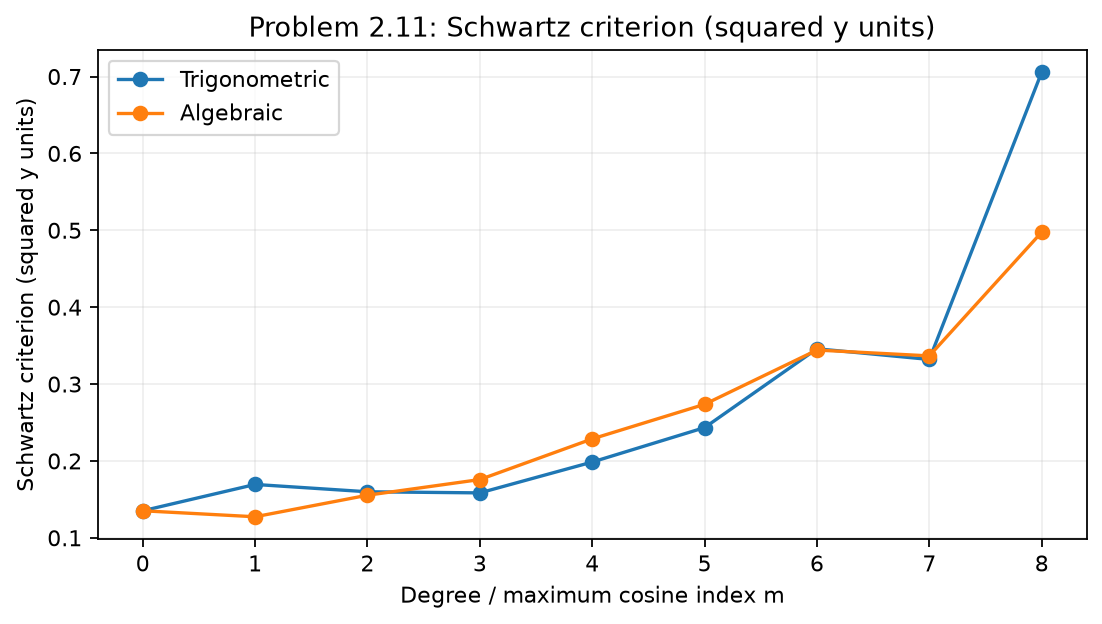
\includegraphics[width=0.88\linewidth]{problem_2_11_criterion.png}
\caption{Complexity selection: choose the lowest point on each family's curve. Blue denotes the cosine (trigonometric) family; orange denotes the algebraic family.}
\end{figure}

\textbf{Why is algebraic $m=1$ selected instead of $m=2$?}
\begin{center}\begin{tabular}{crr}
\toprule
$m$ & Training MSE & Schwartz score\\\midrule
1 & 0.08084 & \textbf{0.12738}\\
2 & 0.07822 & 0.15541\\\bottomrule
\end{tabular}\end{center}
Adding the quadratic term slightly improves the training fit, but the improvement does not offset the larger complexity multiplier. The criterion therefore prefers the line.

\textbf{What limits the cosine family?} Every basis function obeys
$\cos(2\pi j(1-x))=\cos(2\pi jx)$ for integer $j$. Hence every fitted cosine model is symmetric about $x=1/2$, while $x^2+0.1x$ is not. Increasing $m$ does not remove this structural restriction. Equal coefficient counts do not make the two model families equally suited to the signal.

\clearpage
\section*{Problem 2.12: How validation is organized}
The ten observations are split using five-fold cross-validation with shuffling and random state 42. Each round uses eight training observations and two held-out validation observations. Both families use the same folds.

\begin{figure}[h!]\centering\small
\setlength{\tabcolsep}{8pt}
\begin{tabular}{c|*{10}{c}}
 &\multicolumn{10}{c}{Sample ID (original order)}\\
Fold&0&1&2&3&4&5&6&7&8&9\\\hline
1&\train&\val&\train&\train&\train&\train&\train&\train&\val&\train\\
2&\val&\train&\train&\train&\train&\val&\train&\train&\train&\train\\
3&\train&\train&\val&\train&\train&\train&\train&\val&\train&\train\\
4&\train&\train&\train&\train&\val&\train&\train&\train&\train&\val\\
5&\train&\train&\train&\val&\train&\train&\val&\train&\train&\train\\
\end{tabular}
\caption{Actual fold assignments. T denotes training and V denotes validation. Each sample is validated once. The two V observations in a row do not participate in fitting or selecting $m$ for that row.}
\end{figure}

\subsection*{Repeat this procedure for each fold}
\begin{center}
\fcolorbox{blue}{pale}{\parbox{0.90\linewidth}{\centering
\textbf{8 training observations}\\[4pt]
For each family, fit all $m=0,\ldots,6$\\
$\Downarrow$\\
Select $m$ using the training-only Schwartz score\\
$\Downarrow$\\
Predict the 2 held-out observations and compute validation MSE
}}
\end{center}
The training size is now 8, so $m+1<8$ limits the search to $m\le6$. The full-data $m$ from Problem 2.11 is not reused. This evaluates the entire fitting-and-selection procedure.

\begin{equation}
\mathrm{MSE}_r=\frac{1}{2}\sum_{i\in V_r}
\bigl[y_i-\widehat f_{T_r}(x_i)\bigr]^2,
\qquad \mathrm{CV\ MSE}=\frac15\sum_{r=1}^{5}\mathrm{MSE}_r.
\end{equation}
Because all validation folds have size 2, the mean fold MSE also equals the MSE over all ten out-of-fold predictions.

\begin{center}\begin{tabular}{crrrr}
\toprule
Fold & Cosine $m$ & Cosine MSE & Algebraic $m$ & Algebraic MSE\\\midrule
1 & 0 & 0.01793 & 1 & 0.02860\\
2 & 0 & 0.14729 & 6 & 942.63846\\
3 & 5 & 0.40218 & 3 & 0.33297\\
4 & 0 & 0.24554 & 0 & 0.24554\\
5 & 0 & 0.20666 & 0 & 0.20666\\\bottomrule
\end{tabular}\end{center}

\clearpage
\section*{Problem 2.12: Results and interpretation}
\begin{figure}[h!]\centering
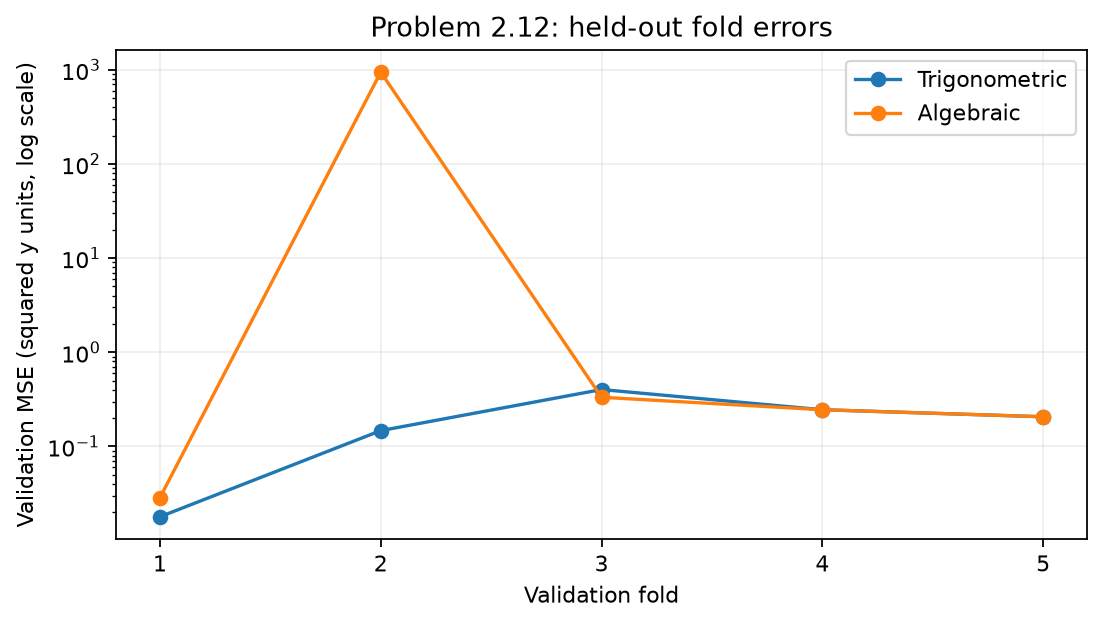
\includegraphics[width=0.72\linewidth]{problem_2_12_folds.png}
\caption{Held-out error by fold. The logarithmic vertical axis reveals both the ordinary errors and the very large algebraic error in fold 2.}
\end{figure}
\begin{figure}[h!]\centering
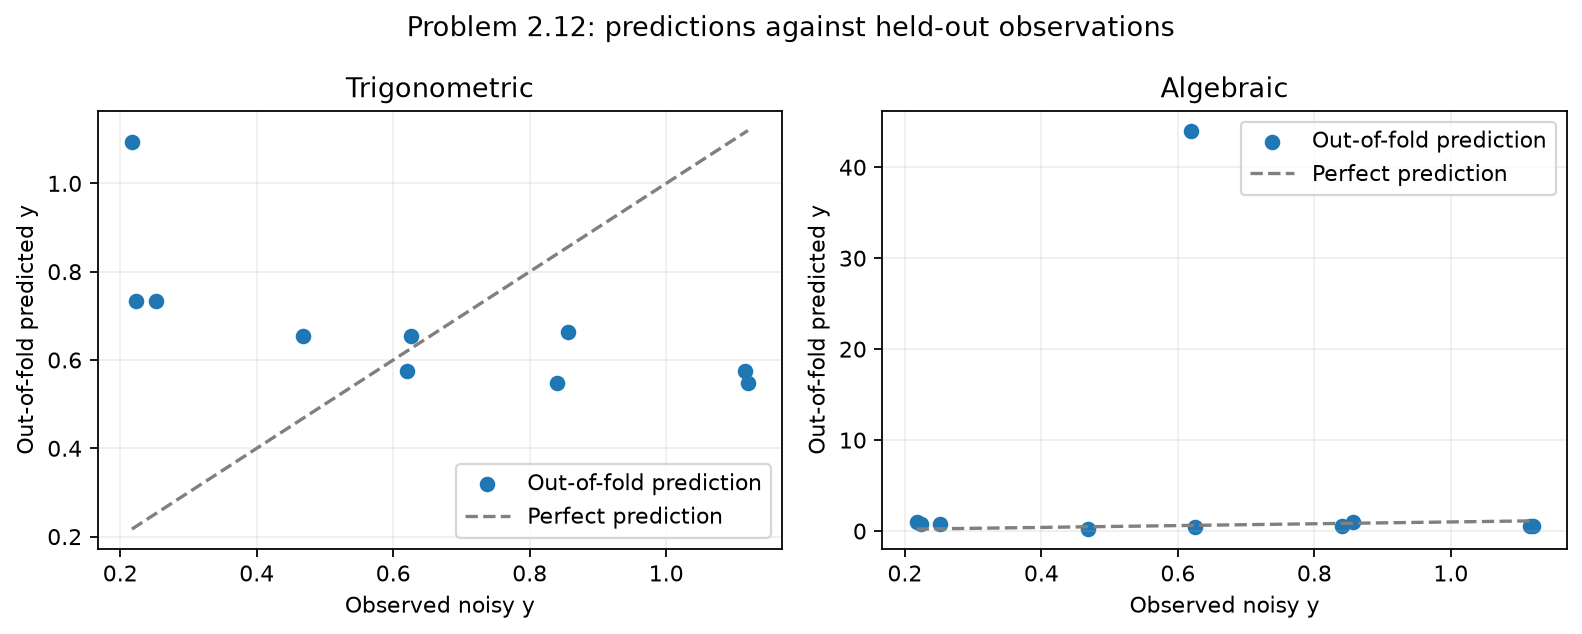
\includegraphics[width=0.82\linewidth]{problem_2_12_oof.png}
\caption{Out-of-fold predictions versus observed responses. The dashed diagonal indicates perfect prediction. The panels use different vertical scales: the algebraic panel exposes the extreme prediction rather than clipping it.}
\end{figure}
\begin{center}\small\begin{tabular}{lrr}
\toprule
Family & Mean validation MSE & Sample SD across folds\\\midrule
Cosine & 0.20392 & 0.14040\\
Algebraic & 188.69045 & 421.46977\\\bottomrule
\end{tabular}\end{center}
\textbf{Interpretation.} The cosine procedure performs better in this particular split. The algebraic mean is dominated by fold 2, where training-only selection chooses $m=6$ from just eight observations. At $x=0.97562$, it predicts $44.03538$ for an observed response of $0.61975$; the fold MSE is 942.64. A flexible fit can have a small training criterion yet predict poorly on held-out observations.

\textbf{Conclusion.} Problem 2.11 favors the algebraic family by its full-data criterion value, while Problem 2.12 favors the cosine procedure by held-out MSE. These are different assessments. Ten observations and one five-fold split provide limited evidence; the results do not establish universal superiority of either family. For KNN, the cross-year results likewise show the limits of obesity as a single predictor of the supplied election labels.
\end{document}
